\documentclass[notes]{beamer}
\usetheme{Madrid}
\usepackage[utf8]{inputenc}
\usepackage{amsmath}
\usepackage{amsfonts}
\usepackage{amssymb}
\newcounter{saveenumi}
\newcommand{\seti}{\setcounter{saveenumi}{\value{enumi}}}
\newcommand{\conti}{\setcounter{enumi}{\value{saveenumi}}}

\resetcounteronoverlays{saveenumi}
%\author{}

\usepackage{geometry} 
\usepackage{array}
\usepackage{float}
\usepackage{placeins}
\usepackage{xcolor}
\usepackage{cancel}
\usepackage{graphicx}
\usepackage{tikz} 
\usepackage[overlay]{textpos}
\usepackage{hyperref}
\usepackage{animate}
\usepackage{wasysym}
\usepackage{listings}

 
 
\newcommand{\tikzmarkk}[2][minimum width=6cm,minimum height=1.5cm]{
 \tikz[remember picture,overlay]
 \node[anchor=west,
       inner sep=0pt,
       outer sep=6pt,
       xshift=-0.5em,
       yshift=-3ex,
       #1](#2){};
}

\newcommand{\shownode}[1]{
  \tikz[remember picture,overlay]\draw[red](#1.south east)rectangle(#1.north west);
}

\newcommand{\showanchor}[1]{
  \tikz[remember picture,overlay]\draw[red,thick,mark=x] plot coordinates{(#1)};
}

% original code from Stefan Kottwitz
% http://tex.stackexchange.com/a/12551/13304
\newenvironment<>{varblock}[2][.9\textwidth]{%
  \setlength{\textwidth}{#1}
  \begin{actionenv}#3%
    \def\insertblocktitle{#2}%
    \par%    
    \usebeamertemplate{block begin}%
    }
  {\par%
    \usebeamertemplate{block end}%
  \end{actionenv}}

\newenvironment{myblock}[1]{\begin{textblock*}{500pt}(#1)}{\end{textblock*}}

% special way to reach the top of the block
\def\newabove(#1){
([yshift=1.5ex]#1.center)
}

\definecolor{dgreen}{rgb}{0.,0.6,0.}
\colorlet{dgr}{green!70!black}
\definecolor{aqua}{rgb}{0.0, 0.2, 1.0}

 
\definecolor{persianindigo}{rgb}{0.2, 0.2, 0.7}  
\newcommand{\indigo}[1]{\textcolor{persianindigo}{#1}}

\definecolor{red}{rgb}{1.0, 0.0, 0.0}  
\newcommand{\red}[1]{\textcolor{red}{#1}}

\title{MicMac V1/V2 état d'avancement}
\subtitle{\textcolor{lightgray}{Ajustement de faisceaux}}
\author{Marc Pierrot Deseilligny 
%\footnotesize \textit{with support slides from A Pinte and M Pierrot Deseilligny}
} 

\institute
{
	Univ. Gustave Eiffel -- IGN/ENSG, LaSTIG lab.- France 
}

\date{novembre 2022}

\graphicspath{{./img/}}

%vertical curmy braces 
\usetikzlibrary{decorations.pathreplacing,calc}
\newcommand{\tikzmark}[1]{\tikz[overlay,remember picture] \node (#1) {};}
  
\begin{document}

\begin{frame}
\titlepage
\end{frame}

\begin{frame}
\tableofcontents
\end{frame}

%%%%%%%%%%%%%%%%%%%%%%%%%%%%%%%%%%%%%%%%%%%%%%%%%%%%%%
\section{MicMac V1 et V2}
%%%%%%%%%%%%%%%%%%%%%%%%%%%%%%%%%%%%%%%%%%%%%%%%%%%%%%

  % -----------------------------------------------------------------
\subsection{Historique  V1}


  %   -  -  -  -  -  -  -  -  -  -  -  -  -  -  -  -  -  -  -  -  -  -  -  -

\begin{frame}{Quelques jalons(1)}
\begin{enumerate}
    \item[2003]  code d'appariement d'images pour les MNS/MNT : multi-échelle, multi-images ;
                 pour l'orientation utilise {\tt OriLib}, modèle {\tt Grille};
    \item[2005]  ajout de méthode d'orientation et d'ajustement pour la calibration géométrique des
                 caméras numériques du LoEMI;
    \item[2007]  intégration des point SIFT comme points homologues , pipeline d'orientation automatique
                 à partir d'un "paquet" d'images:
    \item[2008]  début d'une collaboration structurante avec le MAP-CNRS dans le domaine du patrimoine;
    \item[2009]  intégration des modèle fisheye (+- "tous" les modèles)
    \item[2010]  diffusion assez large de MicMac dans différentes communautés scientifiques (patrimoine, environnement)
\end{enumerate}
\end{frame}

  %   -  -  -  -  -  -  -  -  -  -  -  -  -  -  -  -  -  -  -  -  -  -  -  -
\begin{frame}{Quelques jalons(2)}
\begin{enumerate}
    \item[2011]  pipeline de calcul de modèles en "vrai 3D" en $100\%$ automatique ,  (i.e, pas   du $2.5$ d):
    \item[2012]  début d'une collaboration structurante en science de la terre avec l'IPGP;
    \item[2013]  portage sous Windows;
    \item[2015]  prise en compte de l'ajustement de faisceau sur des capteurs satellitte;
    \item[2018]  \dots décision de lancer une deuxième version $V_2$.
    \item[2020]  début de recherches utilisant le deep learning dans $V_1$;
\end{enumerate}
\end{frame}

  %   -  -  -  -  -  -  -  -  -  -  -  -  -  -  -  -  -  -  -  -  -  -  -  -
\begin{frame}{Bilan-1 Points positifs }
\begin{enumerate}
    \item  une chaine photogrammétrique libre open source complète  (satellite, aérien, terrestre)  
    \item  une chaine photogrammétrique centrée sur la métrologie, offrant un contrôle fin des étapes de calcul (!= boite noire);
    \item  un outil qui a été largement utilisé à l'IGN (calcul de MNS France par la production,  études à IGN-Espace, 
           apprentissage de la photogrammétrie à l'ENSG, prestation en photogra terrestre par le SGM, utilisation 
           au Matis/Lastig);
    \item  a été largement utilisé par des scientifiques, ingénieur \dots dans le patrimoine et l'environnement (2010-2016) ;
    \item  a été financé par plusieurs acteurs privés ou public ($4$ thèses industrielles, $1$ ANR, $1$ FUI, projet CNES-TOSCA).
\end{enumerate}
\end{frame}


  %   -  -  -  -  -  -  -  -  -  -  -  -  -  -  -  -  -  -  -  -  -  -  -  -
\begin{frame}{Bilan -2 , points negatifs}

Un outil qui s'est dévloppé depuis $15$ ans, sans réelle stratégie globale, et pour l'essentiel avec 
un seul programmeur pour le noyau. Conséquences :

\begin{enumerate}
    \item  une chaine sans interface et compliquée à utiliser : noms de commandes sans rapport avec ce qu'elles font,
           message d'erreur peu clairs

    \item un code peu ou mal documenté; pas de test unitaire, fonctionnel ; 

    \item des choix de conception complexes, notamment des optimisation (CPU, mémoire) moins justifiées avec le 
          matériel actuel; le gros de la librairie est orientée traitement d'image, alors que l'usage majoritaire est photogrammétrique;

    \item  utilise peu de librairies externes, beaucoup de "home made" sur des fonctionnalité courante (lecture tiff maison,
           certaines interface sur XLib);

    \item  des contribution externes réalisées par des contractuels, pas facile à maintenir;

    \item  une chaine "viellissante" à l'ère du deep-learning, big data .
\end{enumerate}

\end{frame}

  %   -  -  -  -  -  -  -  -  -  -  -  -  -  -  -  -  -  -  -  -  -  -  -  -
\begin{frame}{Décisions}

     MicMac V1 ne pourra pas évoluer sur le long terme :
      
\begin{enumerate}
    \item  soit on "abandonne" à moyen terme, en se limitant à une maintenance currative;
    \item  soit on fait une nouvelle version.
\end{enumerate}

\pause

\vline

    Il y a un interet a avoir une chaine photogrammetrique open source  complete développée à l'IGN
    En faisant une deuxième itération grace au recul, on espère reprendre les bonnes idées et éviter  les ecueil de V1.

\begin{enumerate}
    \item  on n'abandonne pas et on fait une nouvelle version!
\end{enumerate}

\end{frame}

  % -----------------------------------------------------------------
\subsection{Le "projet" MicMac V2}


  %   -  -  -  -  -  -  -  -  -  -  -  -  -  -  -  -  -  -  -  -  -  -  -  -
\begin{frame}{Ulisateurs  prioritaires}

Utilisateurs  prioritaires :

\begin{enumerate}
    \item  étudiants et enseignants en photogrammétrie, notamment ENSG;

    \item  chercheurs en STIC utilisant la photogrammétrie, notamment au LaSTIG, CEREMA, UGE \dots

    \item  expert/ingénieur en photogrammétrie terrestre, aérienne et spatiale, notamment à l'IGN
           et dans le cadre de collaborations formalisées(CERN).
\end{enumerate}

\vline

$\rightarrow$ Les utilisations plus "grands publics" pour avoir des modèles visuellement  plaisants
ne sont pas une priorité, mais pourront se développer dans le cadre de collaborations (ex
développement pour les archives dans le cadre du stage d'Alexane NGhien).

\end{frame}

  %   -  -  -  -  -  -  -  -  -  -  -  -  -  -  -  -  -  -  -  -  -  -  -  -
\begin{frame}{Les "interfaces"}

\begin{enumerate}
     \item {\bf programmeur}, au niveau du code lui-même pour les programmeurs, avec objectif d'avoir une qualité de code et
           de documentation le permettant;

     \item {\bf expert},  au niveau ligne de commandes : noms rationnels, complétions automatique, spécifications des
                    commandes (entrée, sortie, objectif);

     \item {\bf étudiant},  vCommand systématisée

     \item {\bf expert,étudiant},  binding python permettant un accès relativement simple, à "grain plus fin" que les commandes;

     \item {\bf "grand public"},  dans le cadre de collaboration extérieur, interface finalisée, contacts pris avec Map-CNRS et
          meshroom.

\end{enumerate}

\end{frame}

  %   -  -  -  -  -  -  -  -  -  -  -  -  -  -  -  -  -  -  -  -  -  -  -  -
\begin{frame}{Organisation : table rase \dots}

\begin{enumerate}
    \item  évolution progressive incompatible avec les ambition de correction des problèmes
    \item  on part "from scratch"  
\end{enumerate}

\pause
\vline
\dots ou presque, il y a provisoirement des liens avec V1 :

\begin{enumerate}
    \item  on link avec V1, qui est utilisé comme librairie externe pour quelques fonctionnalités avant
           que l'on  choisisse la "bonne" lib (essentiellement lecture/ecriture des images);


    \item  on peut importer des données V1 au format V2 pour prototyper des chaines complètes (exemple dévloppement de surfaces
           pour les archives nationales);

    \item  on peut faire du copié-collé de code sur des petits morceaux autonomes (marginal).

\end{enumerate}

\end{frame}

  %   -  -  -  -  -  -  -  -  -  -  -  -  -  -  -  -  -  -  -  -  -  -  -  -
\begin{frame}{Organisation : équipe \dots}

Actuellement un peu plus de $2$  ETP . A gros traits :

\begin{enumerate}
   \item  Mehdi Daakir, dans le cadre du CERN, test Window, développemet de tests fonctionnels;
   \item  Celestin Huet, dans le cadre du CERN, développement spécifique, ajout de librairies externes;
   \item  Yann Meneroux, détection de cibles pour PRISMA
   \item  Christophe Meynard, informatique  (portage windows, git, vcommand et complétion), dérivée formelle (avec MPD);
   \item  Jean Michaël Muller, binding python, ajout de la topographie;
   \item  Marc Pierrot Deseilligny, développement du noyau;
   \item  Ewelina Rupnik, estimation de pose  initiale rapide et précise.
\end{enumerate}

\end{frame}

  %   -  -  -  -  -  -  -  -  -  -  -  -  -  -  -  -  -  -  -  -  -  -  -  -
\begin{frame}{Etat d'avancement, général}

\begin{enumerate}
    \item  noyau ($70\%$ ??) : classe pour les commandes, la gestion de chantier, la serialization,
           les dérivées partielles, l'optimisation non linéaire, 


    \item  portage windows, ok en interne, premier beta testeur CERN en janvier;

    \item  vCommand et complétion, premier proto,  en beta;  binding python : premiers exercices avec les PPMD hier !

    \item  tests unitaires : $80\%$ 

    \item  tests fonctionnel  : $40\%$ 

    \item  documentation algorithmique ($60\%$ ??) de l'existant

    \item  documentation programmeur à haut niveau  ($50\%$ ??) de l'existant

    \item  documentation programmeur  dans le code  ($70\%$ ) .


\end{enumerate}
\end{frame}

  %   -  -  -  -  -  -  -  -  -  -  -  -  -  -  -  -  -  -  -  -  -  -  -  -
\begin{frame}{Etat d'avancement, thématique}

\begin{enumerate}
    \item  détection de cible codées, pour l'IGN et le CERN : $90\%$;

    \item  classe capteur avec perspective central quasi complet, incluant plusieur modèle 
           de fishey et de nombreux modèle de distorsion;

    \item  estimation de poses initiales : relèvement dans l'espace (calibré ou non),
           matrice essentielles;
    

    \item  ajustement de faisceau, assimilation de : points d'appuis, points de liaison,
           contraintes de bloc rigide,  inclinomètres ($70\%$) ; possibilité de contrainte

    \item  développement de surface;
\end{enumerate}
\end{frame}

%%%%%%%%%%%%%%%%%%%%%%%%%%%%%%%%%%%%%%%%%%%%%%%%%%%%%%
\begin{frame}
\section{Ajustement de faisceaux}

\begin{center}
{\bf {\Large Ajustement de faisceaux}}
\end{center}

\end{frame}
%%%%%%%%%%%%%%%%%%%%%%%%%%%%%%%%%%%%%%%%%%%%%%%%%%%%%%

  %   -  -  -  -  -  -  -  -  -  -  -  -  -  -  -  -  -  -  -  -  -  -  -  -
\begin{frame}{Equation de projection}

Equation "principale", de projection classique  avec les notations ;

\begin{enumerate}
    \item  le point  terrain  $P_j$ visible and $k$
    \item  le senseur  $k$ avec une fonction de projection terrain-image $\pi_k$;
    \item  le point  image  $q_{j,k}$ visible and $k$
\end{enumerate}

Pour tous les point où  $P_j$ est visible dans $\pi_k$ :

\begin{equation}
    \pi_k (P_j) = q_{j,k} \label{EqPrinc}
\end{equation}

Ici $\pi_k$  est inconnu, $q_{j,k}$ est une observation et $P_j$  peut être suivant les cas :

\begin{enumerate}
    \item  une observation ;
    \item  une inconnue avec des observations;
    \item  une inconnue sans obervation (point de liaison multiple ou non).
\end{enumerate}


\end{frame}

  %   -  -  -  -  -  -  -  -  -  -  -  -  -  -  -  -  -  -  -  -  -  -  -  -

\begin{frame}{Formalisation}

En plus de l'équation "principale" \ref{EqPrinc}, on un certain nombre d'équation auxiliaires
.(bloc, GPS \dots) non détaillées ici $A_i$.  Comme on a (beaucoup) plus d'inconnues que d'équations ,
on formalise le problème par moindre carrés :

\begin{equation}
    \sum_{j,k}  |\pi_k (P_j) - q_{j,k} |^2  + \sum_i A_i^2  \label{EqLstSq}
\end{equation}

Comme le système n'est pas linéaire on le linéarise par différenciation. 

Comme la linérisation est une approximation on itère.

\end{frame}

  %   -  -  -  -  -  -  -  -  -  -  -  -  -  -  -  -  -  -  -  -  -  -  -  -

\begin{frame}{Implementation}

Le diable est dans les détails \dots Il reste à définir notamment :

\begin{enumerate}

   \item comment calculer les dérivées;

   \item comment stocker  les systèmes de moindres carrés;

   \item comment gérer les grands systèmes avec des $10^4 \dots 10^6$ points de liaisons;

   \item comment résoudre les systèmes de moindres carrés;

   \item quel modèles de caméra;
\end{enumerate}

\end{frame}

  %   -  -  -  -  -  -  -  -  -  -  -  -  -  -  -  -  -  -  -  -  -  -  -  -

\begin{frame}{Calcul des dérivées-1}

Les principales méthodes de calcul des dérivées sont :

\begin{enumerate}
    \item à la main  ; $+$ efficace ,  $-$ source d'erreur, difficile à maintenir; 

    \item  dérivées numérique  ; $+$ simple, $-$ lent, risque d'imprécision;

    \item  jet  : $+$ exact  , $-$ un peu lent , un peu compliqué à développer 
           (NB un jet = 1 nombre + un infiniment petit formel, voir  CERES)

    \item   dérivées symboliques : $+$ exact et rapide , $-$ moyennement compliqué à développer (mais assez simple à utiliser)

    \item   code differenciation : $+$ exact et rapide, permet de dériver des expression avec des boucles 
            $-$ très compliqué à développer et assez compliqué à utiliser.
\end{enumerate}

La méthode utilisée dans MicMac  (V1 et V2) est celle des dérivées symboliques.

\end{frame}

  %   -  -  -  -  -  -  -  -  -  -  -  -  -  -  -  -  -  -  -  -  -  -  -  -

\begin{frame}{Calcul des dérivées-2}

Représentation des formules comme un arbre :

\begin{figure}
   \centering
	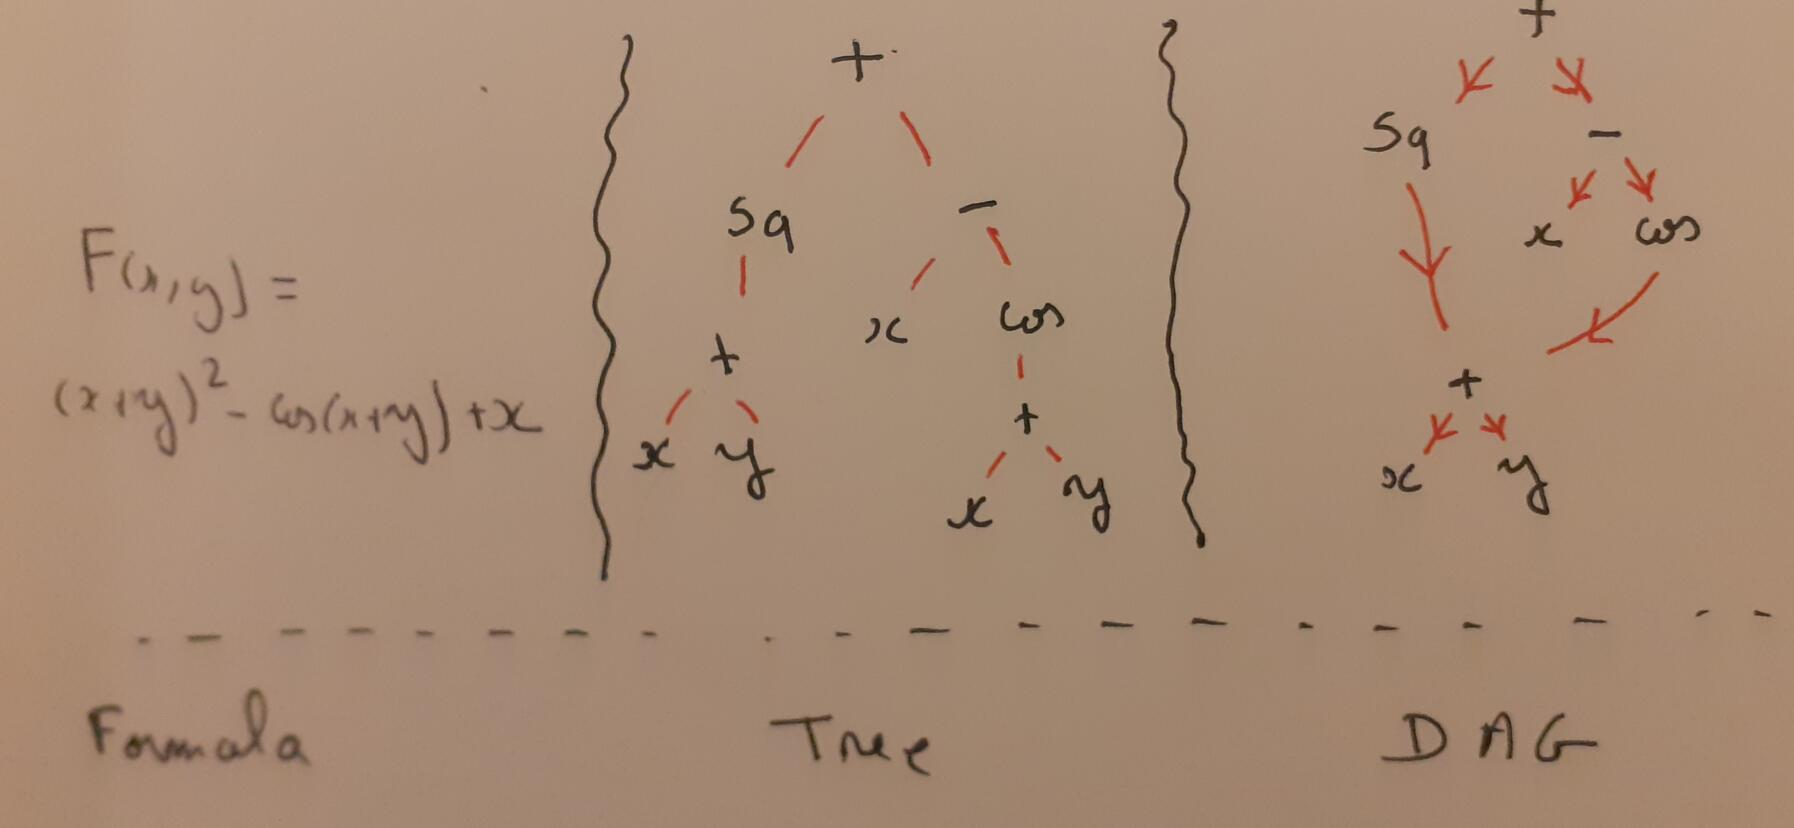
\includegraphics[width=0.5\textwidth]{../Programmer/ImagesProg/Tree.jpg}
   \label{fig:chambre_noire_pic}
\end{figure}

On définit toute les opérations sur les arbres de formules.

\end{frame}

  %   -  -  -  -  -  -  -  -  -  -  -  -  -  -  -  -  -  -  -  -  -  -  -  -

\begin{frame}[fragile]{Calcul des dérivées-3}

{\tiny

\begin{lstlisting}[language=c++]

begin{lstlisting}[language=c++]
// === Extract of code in class cMulF (multiplication of formulas )

// method for computing values
void ComputeBuf(int aK0,int aK1) override
{
    for (int aK=aK0 ; aK<aK1 ; aK++)
        mDataBuf[aK] =  mDataF1[aK] * mDataF2[aK];
}

// method for computing the derivative
cFormula<TypeElem> Derivate(int aK) const override
{
   return  mF2*mF1->Derivate(aK) + mF1*mF2->Derivate(aK);
}

// method for generating the code
std::string GenCodeDef() const override
{
    return "(" + mF1->GenCodeRef() + " " + this->NameOperator() +  " " + mF2->GenCodeRef() + ")";
}
\end{lstlisting}

}

\end{frame}

  %   -  -  -  -  -  -  -  -  -  -  -  -  -  -  -  -  -  -  -  -  -  -  -  -

\begin{frame}{Calcul des dérivées-4}

Les formules identiques sont identifiées, le code est représenté comme un DAG :

\begin{figure}
   \centering
	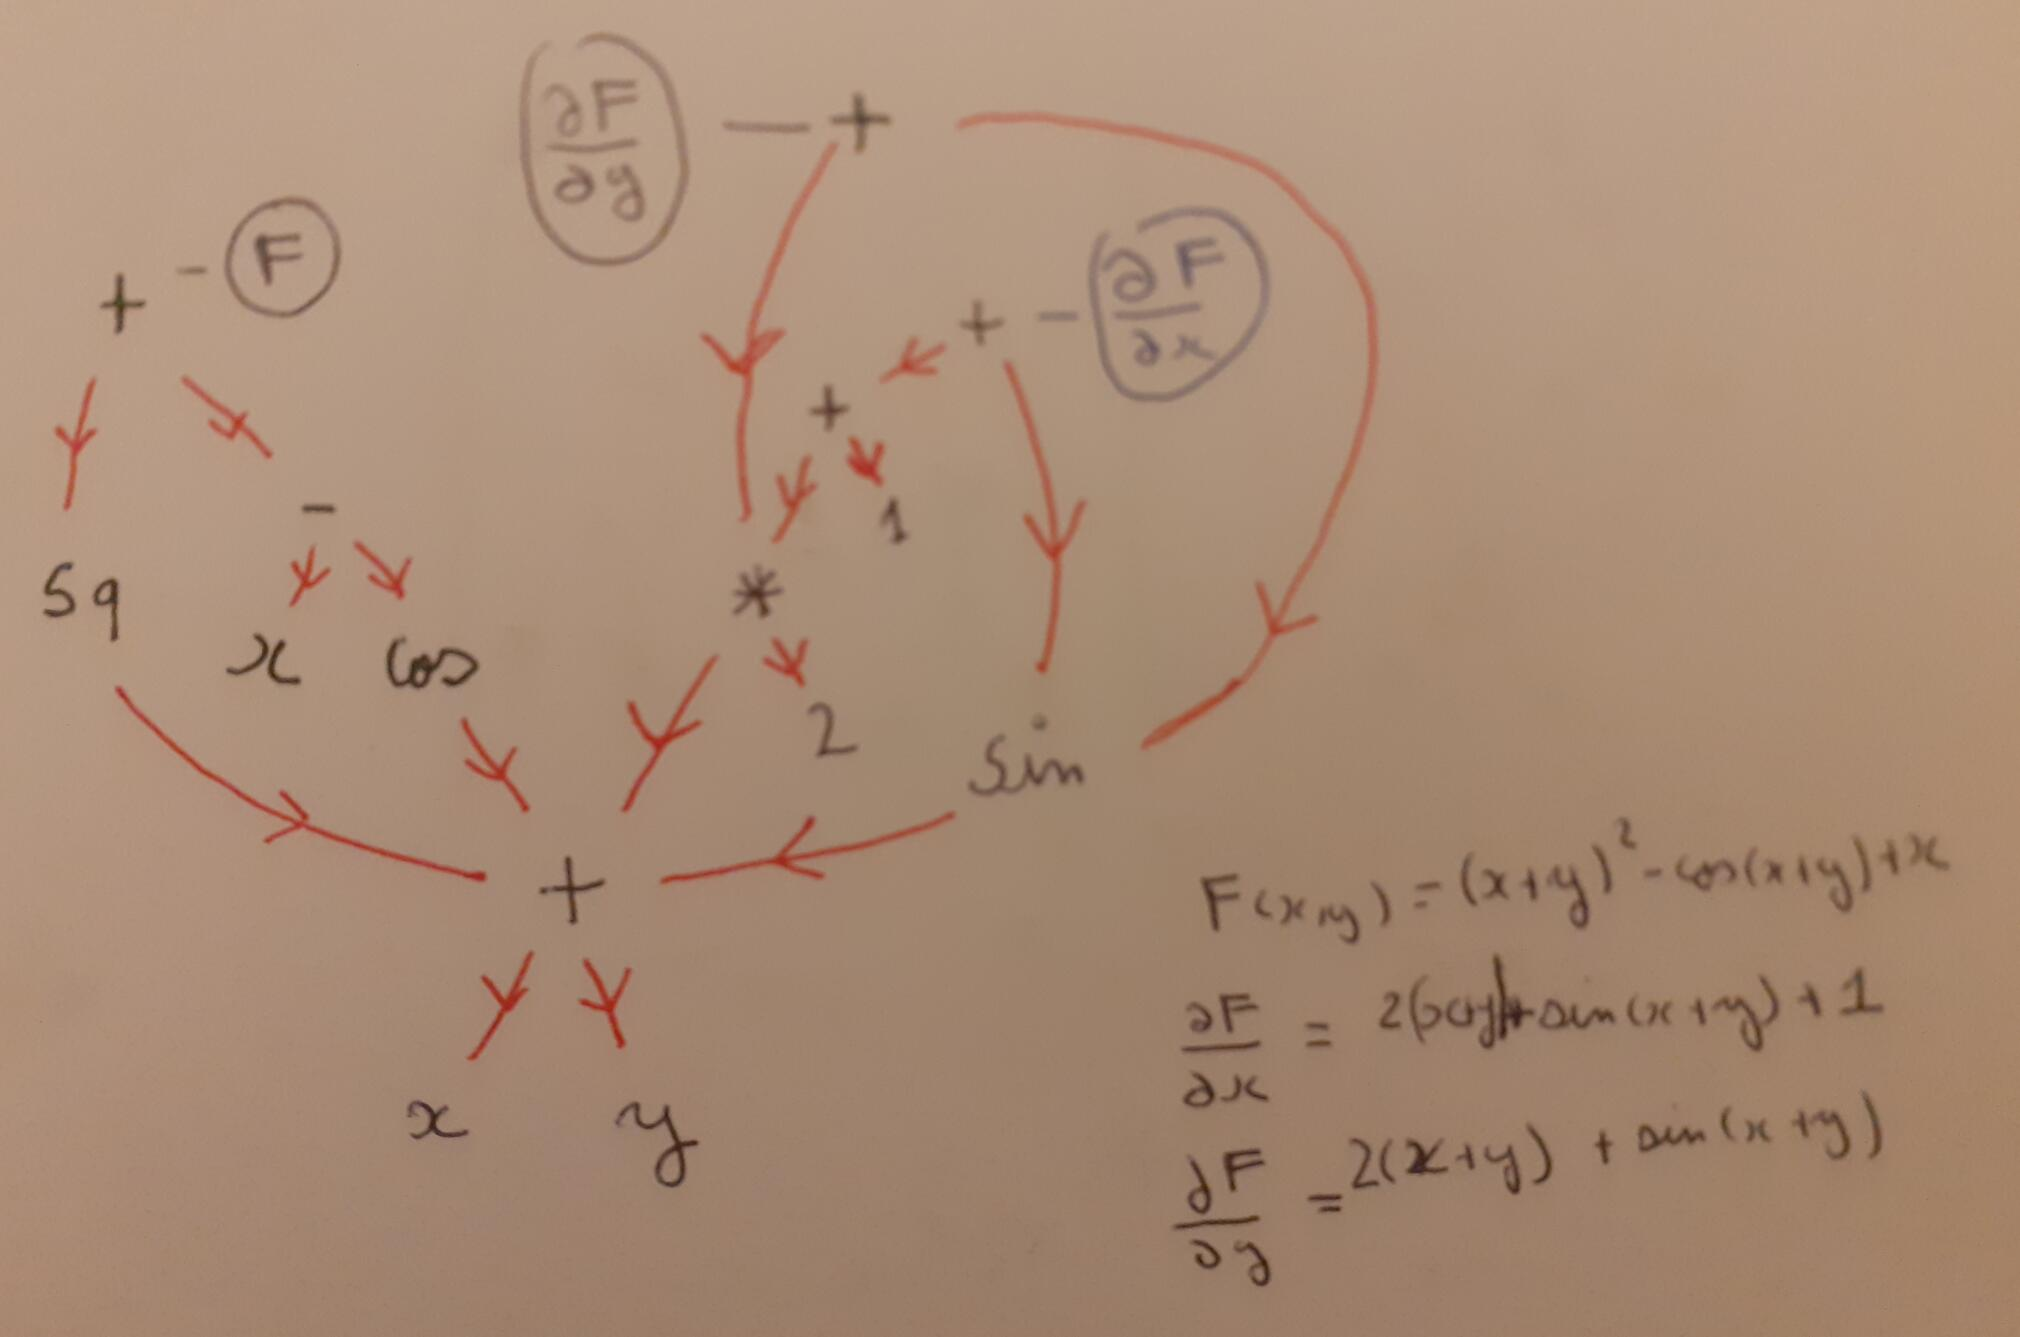
\includegraphics[width=0.5\textwidth]{../Programmer/ImagesProg/DAG.jpg}
   \label{fig:chambre_noire_pic}
\end{figure}


\end{frame}

  %   -  -  -  -  -  -  -  -  -  -  -  -  -  -  -  -  -  -  -  -  -  -  -  -

\begin{frame}{Calcul des dérivées-5}

{\tiny 
Les principales règles de réductions sont utilisées :

\begin{itemize}
     \item  $0*F \rightarrow 0$ ,   $1*F  \rightarrow F$ , $-1*F \rightarrow -F$ (and idem $F*0\dots$);

     \item  $0/F \rightarrow 0$ ;

     \item  $0+F \rightarrow F$ ,   (and idem $F+0\dots$);

     \item  $-(-F) \rightarrow F$ ,  $F_1-(-F_2) \rightarrow F_1+F_2$;

     \item  $F_1*F_2 + F_1*F_3  \rightarrow F_1*(F_2+F_3)$ , $F_1*F_2 - F_1*F_3  \rightarrow F_1*(F_2-F_3)$ ,
     \item  $F_2/F_1 + F_3/F_1  \rightarrow (F_2+F_3)/F1$ ,  $F_2/F_1 - F_3/F_1  \rightarrow (F_2-F_3)/F1$ ,

     \item if  $F_1 > F_2$ then  $F_1 + F_2  \rightarrow F_2 + F_1$ , here the comparison $F_1 > F_2$
           is made on numbering, this rules is here favorize merging in DAG creation , any comparison as long
           as it anti-symetric would hold; we just want to avoid that in the same formula $F_1+F_2$ and $F_2+F_1$
           cannot be merged;
     \item if  $F_1 > F_2$ then  $F_1 * F_2  \rightarrow F_2 * F_1$

     \item  $C(a) \otimes C(b) \rightarrow C(a \otimes b) $  where  $C(x)$ design the formula for constant $x$
             and $\otimes$ is any bynary operator;
     \item  $ \alpha (C(a)) \rightarrow C(\alpha (a)) $  where  $\alpha$ design any unary operator;

\end{itemize}

}

\end{frame}

  %   -  -  -  -  -  -  -  -  -  -  -  -  -  -  -  -  -  -  -  -  -  -  -  -

\begin{frame}{Calcul des dérivées-6}
Le code généré ressemble à quelques chose comme cela :

\vline

{\small
{\tt
    double F29 = std::sin(F8);

    double F13 = MMVII::DerSinC(F8);

    double F14 = (2 * F8);

    double F9 = MMVII::sinC(F8);

    double F16 = (F15 / F14);

    double F10 = (F9 * PixI);

    double F22 = (F21 / F14);

    double F11 = (F9 * PixJ);

    double F18 = (F16 * F13);

    double F32 = -(F22);

    double F24 = (F22 * F13);
}
}


\end{frame}

  %   -  -  -  -  -  -  -  -  -  -  -  -  -  -  -  -  -  -  -  -  -  -  -  -

\begin{frame}{Stockage des obsevations, gestion des grands systèmes, résolution des équations}

La résolution des équation est faite par eigen, le stockage et la réduction est faite en interne.
On note  $^t L_i X = r_i$   une observation .  Pour mémoriser l'ensemble des observations, V2 propose trois option.

{\bf Option 1:} adapatée au cas ou l'on veut calculer les incertitudes et corrélation ;

\begin{enumerate}
    \item on accumule dans une matrice nomale pleine ($\sum Li ^tLi$),
    \item  les inconnue  "inutile" de types points de liaisons sont éliminées par compléments de Schurr, 
    \item  le sytème est résolu avec  {\tt eigen::ldlt} (  Robust Cholesky decomposition of a matrix with pivoting). 
\end{enumerate}
      
\end{frame}
  %   -  -  -  -  -  -  -  -  -  -  -  -  -  -  -  -  -  -  -  -  -  -  -  -

\begin{frame}{Stockage (2)}

{\bf Option 2} option par défaut, adaptée aux grands systèmes d'ajustement :
\begin{enumerate}
    \item on accumule dans une matrice nomale creuse dynamique 
    \item  on utilise le complément de schurr 
    \item  le système est résoly avec  {\tt eigen::SimplicialLDLT}
          (direct sparse LDLT Cholesky factorizations without square root). 
\end{enumerate}

{\bf Option 3} théoriquement recommandée par {\tt eigen} pour sa stabilité :
\begin{enumerate}
    \item on mémorise la liste des équations
    \item  on n'élimine rien
    \item  le système est résolu avec  {\tt eigen::LeastSquaresConjugateGradient}
          (conjugate gradient solver for sparse (or dense) least-square problems). 
\end{enumerate}

\end{frame}

  %   -  -  -  -  -  -  -  -  -  -  -  -  -  -  -  -  -  -  -  -  -  -  -  -

\begin{frame}{Modélisation des caméras, cas aérien}

Beaucoup de modèles de caméra proposé. Un modèle est caractérisé par les paramètres suivants:

\begin{enumerate}
    \item un  type parmi des valeurs énumérées  Sténopé (= "normal"), Fisheye équisolide, Fisheye equidistant, 
          fisheye stéréographique, fisheye orthographique, equirectangulaire (caméra 360)

    \item degré radial ;
    \item degré décentrique;
    \item degré pour les polynômes quelconques.
\end{enumerate}

Par exemple, modèle "standard" de Fraser correspondra : {\tt sténopée} + $3,1,1$,
$3$ pour $R^3,R^5,R^7$, $1$ pour les deux paramètres décentriques $p_1$ et $p_2$,
$1$ pour les deux paramètres affines $b_1$ et $b_2$.


\end{frame}

  %   -  -  -  -  -  -  -  -  -  -  -  -  -  -  -  -  -  -  -  -  -  -  -  -

\begin{frame}{Modélisation des caméras, cas spatial-1}

Pas encore fait dans V2, mais on compte reprendre en partie le même principe que dans V1:


\begin{enumerate}
    \item hypothèse : la position est précise (GPS sans obstruction), l'imprécision vient de l'orientation;
    \item la  correction est une déformation image  lisse, indépendante du relief;
\end{enumerate}

Modèle de projection :

\begin{equation}
   \pi  =  D \circ \pi_0
\end{equation}
On se donne pour $D$ un modèle paramétrique de type polynomial en $x,y$. 
\end{frame}

  %   -  -  -  -  -  -  -  -  -  -  -  -  -  -  -  -  -  -  -  -  -  -  -  -
\begin{frame}{Modélisation des caméras, cas spatial-1}
Eventuellement on le contraint localement à être proche
des rotations , avec $O,P,K $ trois fonctions de $x$ à variation lente.

\begin{equation}
   D  (x,y)  \approx O(x)  \frac {\partial \pi_0} {\partial \omega} + P(x) \frac {\partial \pi_0} {\partial \phi} + K(x)\frac {\partial \pi_0} {\partial \kappa}
   \label{WPK}
\end{equation}

En pratique dans la majorité des chantier traités en recherche (emprise limitée) on se limite au degré 1 en $x,y$ et on n'utilise peu~\ref{WPK}.
Cette formalisation serait probablement à revoir dans le cadre d'un usage IGN sur de longues bandes.

\end{frame}


%%%%%%%%%%%%%%%%%%%%%%%%%%%%%%%%%%%%%%%%%%%%%%%%%%%%%%
\section{Expérimentation sur PVA IGN}
%%%%%%%%%%%%%%%%%%%%%%%%%%%%%%%%%%%%%%%%%%%%%%%%%%%%%%

\begin{frame}
\begin{center}
{\bf {\huge Expérimentation sur PVA IGN}}
\end{center}
\end{frame}

\subsection{Introduction}

  %   -  -  -  -  -  -  -  -  -  -  -  -  -  -  -  -  -  -  -  -  -  -  -  -
\begin{frame}{Motivation}

Contexte de ce travail :

\begin{enumerate}
    \item  sollicitation des développement image (Ana Maria Rosu) pour suivre les évolutions de micmac ;
    \item  interêt de MPD pour voir à quel point micmac V2 pouvait être potentiellement proche ou pas d'une utilisation
           sur des besoins IGN;
    \item  pas de demande de la part du SIA, mais  réponse  très constructives de Benjamin Ferrand aux (nombreuses) questions de MPD
           sur les méthodologies utilisées au SIA .
\end{enumerate}

Quelques ajouts spécifiques fait à MicMac-V2 pour traiter ces chantier. A part, éventuellement des conversion de format,
ce sont des éléments qui étaient sur la feuille de route.  Charge, environ une semaine pour les conversion de format, 1 semaine
pour les ajouts algorithmiques.

\end{frame}


  %   -  -  -  -  -  -  -  -  -  -  -  -  -  -  -  -  -  -  -  -  -  -  -  -
\begin{frame}{Description du chantier}

\begin{center}
\emph{à vérifier par SIA+devimage}
\end{center}

\begin{enumerate}
    \item   prise de vue effectuée par un sous-traitant;
    \item   $2000$ image acquise sur un terrai  plat (somme), caméra vexcel 
    \item   solution de geo-référencemnent directe de "bonne" qualité ($1$-$2$ pixel en relatif  $??$ en absolu);
    \item   $??$  point de liaison calculé par logiciel propriétaire , précision autour de $\frac{2}{10}$ de pixel;
    \item   $40$ point terrain,  a priori tous à utiliser uniquement en controle.
\end{enumerate}

\end{frame}

  %   -  -  -  -  -  -  -  -  -  -  -  -  -  -  -  -  -  -  -  -  -  -  -  -
\begin{frame}{Pipeline de traitement}

\begin{enumerate}
    \item  import des données de trajectographie  orientation $WPK$ + GPS en lambert $93$;
    \item  conversion en un repère tangent local;
    \item  ajustement de faisceau avec différentes options;
    \item  mesure des résidu terrain (moyenne et déviation standard des résidu $3d$);
    \item  éventuellement, retour en lambert $93$.
\end{enumerate}

\end{frame}

  %   -  -  -  -  -  -  -  -  -  -  -  -  -  -  -  -  -  -  -  -  -  -  -  -
\begin{frame}{Options testées de l'ajustement de faisceau}
 
Options testées :
\begin{enumerate}
    \item  avec et sans paramètres additionnels;
    \item  avec et sans libération de la focale et du point principal;
    \item  avec contrainte stricte sur la position GPS ou "soft" contrainte;
\end{enumerate}

L'ajout de bras de levier n'a pas été testé, sur ce terrain "plat" il est quasi équivalent au
couple focale point principal. La prise en compte est a priori facile, ce sont les mêmes equation
que le bloc rigide (déjà ajouté pour le CERN), mais nécessite un peu de gestion de chantier.

\end{frame}

  %   -  -  -  -  -  -  -  -  -  -  -  -  -  -  -  -  -  -  -  -  -  -  -  -
\begin{frame}{Traitement des paramètres additionnels (2)}

Lorsque le SIA ajoute des systématisme de bloc, pour chaque bloc on a deux paramètre $a,b$
qui opèrent ainsi :

\begin{equation}
    \delta_x = ax   ; \delta_y = b x
\end{equation}

Sous micmac-V2, on a rajouté, parce qu'il existait déjà comme modèle de caméra prédéfini ($0,0,1$) 
les paramètres $a,b$ suivant :

\begin{equation}
    \delta_x = b_1  + b_2 y   ; \delta_y = 0
\end{equation}

\end{frame}

  %   -  -  -  -  -  -  -  -  -  -  -  -  -  -  -  -  -  -  -  -  -  -  -  -
\begin{frame}{Traitement des paramètres additionnels(2)}
Si on considère que la focale est libre, et compte tenu de la rotation de la caméra autour de son axe,
ces deux paramètrage engendrent la même famile de fonction (espace vectoriel) avec des bases différentes :

\begin{equation}
       E_1 =
       a \begin{pmatrix} 1 & 0 \\ 0 & 0 \end{pmatrix}
      +b \begin{pmatrix} 0 & 0 \\ 1 & 0 \end{pmatrix}
      +r \begin{pmatrix} 0 & -1 \\ 1 & 0 \end{pmatrix}
      +f \begin{pmatrix} 1 & 0 \\ 0 & 1 \end{pmatrix}
\end{equation}

\begin{equation}
       E_2 =
       b_1 \begin{pmatrix} 1 & 0 \\ 0 & 0 \end{pmatrix}
      +b_2 \begin{pmatrix} 0 & 1 \\ 0 & 0 \end{pmatrix}
      +r \begin{pmatrix} 0 & -1 \\ 1 & 0 \end{pmatrix}
      +f \begin{pmatrix} 1 & 0 \\ 0 & 1 \end{pmatrix}
\end{equation}

On a :

\begin{equation}
       E_1 = E_2
\end{equation}

\end{frame}

  %  -----------------------------------------------------------------------------------------

\subsection{traitement MicMac-V2}

\begin{frame}
\begin{center}
{\bf {\Large Traitement MicMac-V2}}
\end{center}
\end{frame}

  %   -  -  -  -  -  -  -  -  -  -  -  -  -  -  -  -  -  -  -  -  -  -  -  -
\begin{frame}{Import des données}

{\tt {\tiny
MMVII ImportOri trajectographie\_tif.opk NSSXYZWPKS Calib001 InitUPCalVol "AngU=degree" "KIsUp=true"
}}

Importe le fichier GPS/IMU, du format texte au format MicMac :

\begin{enumerate}
    \item  {\tt NSSXYZWPKS}  indique quel colonnes correspondent à quelles données;
    \item  {\tt Calib001}  indique la localisation des données de calibration initiales ;
    \item  {\tt InitUPCalVol}  indique la localisation des données des données de sorties;
    \item  {\tt KIsUp=true}  indique que la convention est que l'axe $K$ est vers le haut;
\end{enumerate}

Importe les GCP :

{\tt {\tiny
MMVII ImportGCP Terrain.APP NSXYZ VolV1 NumL0=1 "ChSys=[Lambert93,RTLProj]"
}}


\end{frame}

  %   -  -  -  -  -  -  -  -  -  -  -  -  -  -  -  -  -  -  -  -  -  -  -  -
\begin{frame}{Calcul d'un répère tangent local}

{\tt {\tiny
 MMVII SysCoCreateRTL VolAllIm.xml Lambert93 RTLProj InOri=InitUPCalVol OutOri=RTLInitUPCalVol Z0=0
}}

\begin{enumerate}
    \item  {\tt VolAllIm.xml}  toute les images; 
    \item  {\tt Lambert93}  indique le système dans lequel sont enregistrées les données;
    \item  {\tt RTLProj}  nom du système de coordonnées créé;
    \item  {\tt InOri=InitUPCalVol}  utilisé pour calculer le centre + crée la conversion;
    \item  {\tt  OutOri=RTLInitUPCalVol}  crée un export;
\end{enumerate}

\end{frame}

  %   -  -  -  -  -  -  -  -  -  -  -  -  -  -  -  -  -  -  -  -  -  -  -  -
\begin{frame}{Compensation}

Ajustement de faisceaux, en figeant les paramètres internes, et en fixant les centre de prises de vues avec un sigma de $0.5$ et un sigma de $1$ pixel;

{\tt {\tiny
MMVII OriBundleAdj VolAllIm.xml RTLInitUPCalVol FixC05\_FrzP DataDir=VolV1  NbIter=3 "TiePWeight=[1]" RefOri=[RTLInitUPCalVol,0.5] PPFzCal=.*
}}

\end{frame}
  %  -----------------------------------------------------------------------------------------

\begin{frame}
\begin{center}
{\bf {\Large Résultats}}
\end{center}
\end{frame}


\subsection{Résultats}

  %   -  -  -  -  -  -  -  -  -  -  -  -  -  -  -  -  -  -  -  -  -  -  -  -
\begin{frame}{Sans systématisme}

\begin{tabular}{ |c|c|c|c|c|c|c|c| }
    \hline
       Mode                              & Pix       & $\mu_x$ & $\mu_y$  & $\mu_z$  & $\sigma_x$ & $\sigma_y$ & $\sigma_z$ \\ \hline
       Init                              & 1.34      & 0.04    & -0.05    &  1.02    &   0.34     &  0.43      &   0.54 \\  \hline
       $\sigma_C=0.5$ $\sigma_I=0.0$     &  0.177341 & 0.02    & -0.02    &  1.16    &   0.35     &  0.4      &   0.33 \\  \hline
 {\bf \red{$\sigma_C=0.5$ $\sigma_I=\infty$}}  &  0.177344 & 0.01    &  0.01    &  0.57    &   0.1      &  0.08      &   0.19 \\ \hline
       $\sigma_C=0.0$ $\sigma_I=0.0$     &  0.220379 & -0.0    & -0.06    &  1.14    &   0.13     &  0.23      &   0.24 \\  \hline
       $\sigma_C=0.0$ $\sigma_I=\infty$  &  0.214886 & 0.01    & -0.02    &  3.79    &   0.09     &  0.09      &   0.21 \\  \hline
     \hline
\end{tabular}
\end{frame}

  %   -  -  -  -  -  -  -  -  -  -  -  -  -  -  -  -  -  -  -  -  -  -  -  -
\begin{frame}{"Trichons" }

Un peu avec un GCP, ou  beaucoup en important la calibration obtenue avec tous les GCP.

\begin{center}
\begin{tabular}{ |c|c|c|c|c|c|c|c| }
    \hline
       Mode                                  & $\mu_x$ & $\mu_y$  & $\mu_z$  & $\sigma_x$ & $\sigma_y$ & $\sigma_z$ \\ \hline
       Fix 462003                            & 0.01    & 0.01    &  0.35    &   0.1     &  0.07      &   0.19 \\  \hline
       Fix 480018                            & 0.01    & 0.00    &  -0.12   &   0.1     &  0.07      &   0.19 \\  \hline
       Calib/GCP                             & 0.01    & 0.00    &  0.007   &   0.1     &  0.09      &   0.19 \\  \hline
     \hline
\end{tabular}
\end{center}

\end{frame}

  %   -  -  -  -  -  -  -  -  -  -  -  -  -  -  -  -  -  -  -  -  -  -  -  -
\begin{frame}{Avec systématismes}

\begin{tabular}{ |c|c|c|c|c|c|c|c| }
    \hline
       Mode                              & Pix       & $\mu_x$ & $\mu_y$  & $\mu_z$  & $\sigma_x$ & $\sigma_y$ & $\sigma_z$ \\ \hline
       $\sigma_C=0.0$ $\sigma_I=\infty$  &  0.214683 & 0.015    & -0.02    &  2.54   &  0.10      &  0.08      &   0.21 \\  \hline
       $\sigma_C=0.5$ $\sigma_I=\infty$  &  0.176569 & -0.02    &  0.02    &  -89    &   0.48     &  0.27      &   0.71 \\ \hline
     \hline
\end{tabular}
\end{frame}


%%%%%%%%%%%%%%%%%%%%%%%%%%%%%%%%%%%%%%%%%%%%%%%%%%%%%%
%%%%%%%%%%%%%%%%%%%%%%%%%%%%%%%%%%%%%%%%%%%%%%%%%%%%%%
%%%%%%%%%%%%%%%%%%%%%%%%%%%%%%%%%%%%%%%%%%%%%%%%%%%%%%

\begin{frame}
\begin{center}
{\bf {\huge Conclusion}}
\end{center}
\end{frame}

\subsection{Conslusion}

  %   -  -  -  -  -  -  -  -  -  -  -  -  -  -  -  -  -  -  -  -  -  -  -  -

\begin{frame}

Le point de vue de la recherche :

\begin{enumerate}
    \item  il y aurait un intérêt à avoir un outil commun  pour l'aéro;

    \item  potentiellement, V2 est assez ouvert pour intégrer les évolutions nécessaires
           aux besoins des autres services IGN;

    \item  potentiellement, V2 est assez bien conçu et documenté pour que les autres services IGN
           puissent y contribuer, au moins cela vaut le coup d'essayer;

    \item  nous avons intérêt du point de vue de la légitimité de V2 à ce que les autres services se l'approprient,
           et donc somme prêt à faire les investissements nécessaires si ils y voient un intérêt.
\end{enumerate}

\end{frame}




\end{document}
